\section{Schaltpläne und PCBs}

Zur Umsetzung des Datenbusses wird für jedes Modul ein Mikrocontroller zur Kommunikation benötigt. 
Über die Mikrocontroller werden die zu verarbeitenden Eingangssignale vom jeweiligen Modul über den Bus an das Controller Modul übertragen. Für die 
unterschiedlichen Funktionen der Module müssen jeweils eigene Platinen entwickelt werden. 


\subsection{Controller Modul}
Der verwendete ESP32 ist wie in Abb. \ref{ESP} verschaltet. Die UART-Bridge wird an den Pins D34 und D35 angeschlossen, da diese al UART Pins vom ESP32 vorgesehen sind. Der interne Datenbus wird an den Pins D13 und D15 angeschlossen, wobei D13 als Receive-Pin und D15 als Transmit-Pin fungiert. Der ESP32 wird über V\textsubscript{in} mit 5V über die USB Spannung versorgt.

\begin{figure}[H]
    \centering    
    \fbox{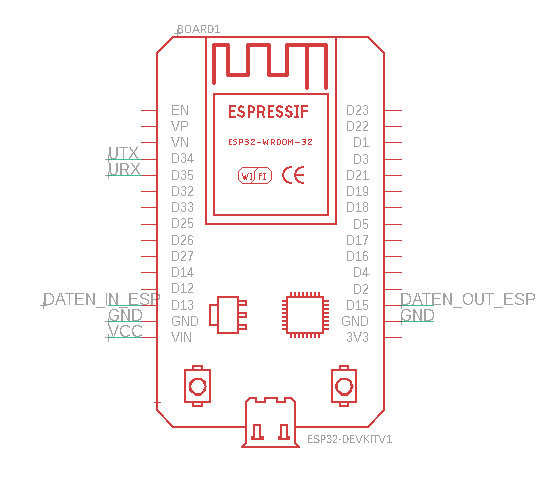
\includegraphics[width=.75\textwidth]{Bilder/ESP.PNG}}
    \caption{ESP32 Verschaltung}
    \label{ESP}
\end{figure}

Für die Kommunikation mit einem PC, werden die Daten über eine UART-Bridge gegeben, bevor sie an die USB Schnittstelle übertragen werden. D+ und D- sind in diesem Fall die USB-Datenleitungen, welche über eine USB-Buchse herausgeführt werden. Die UART-Datenleitungen vom ESP32 zur UART-Bridge sind in \ref{USB} verdreht, da es sich um die Labels aus Sicht des ESP32 handelt.


\begin{figure}[H]
    \centering    
    \fbox{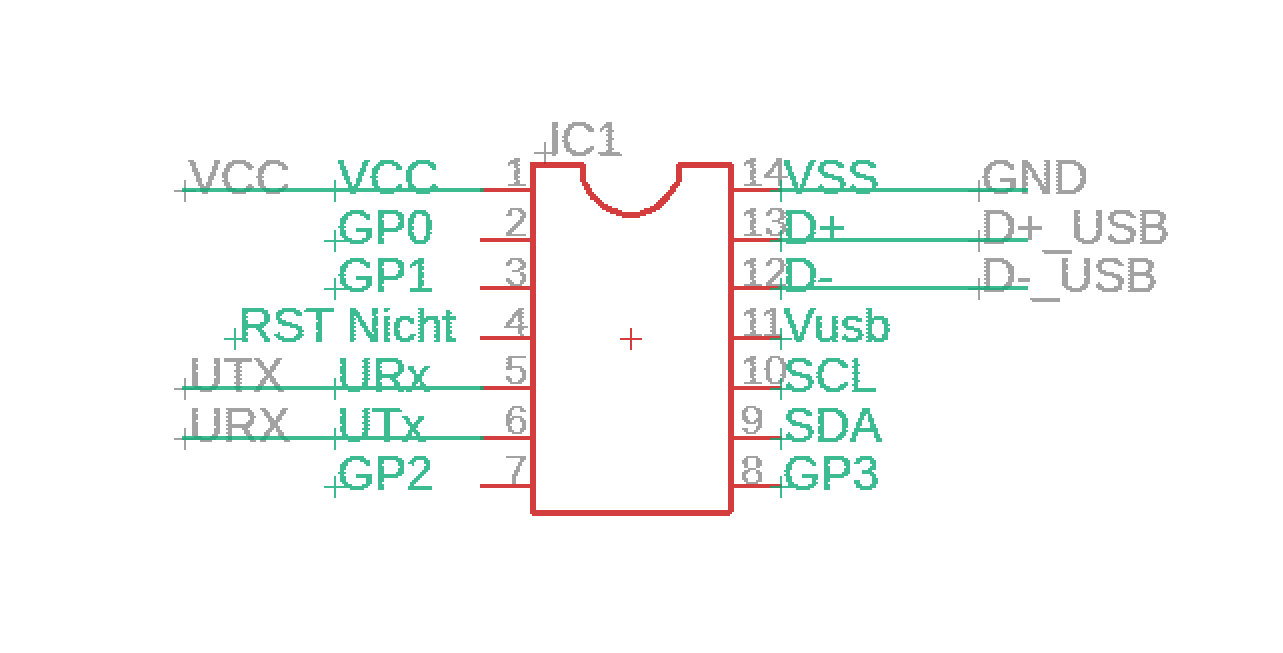
\includegraphics[width=.8\textwidth]{Bilder/BU_USB.PNG}}
    \caption{UART-Bridge}
    \label{USB}
\end{figure}

Zur Kommunikation auf unserem Datenbus werden die Daten differenziell übertragen. Welches über den Transmitter SN65LVS1D und den Receiver SN65LVDT2D passiert.

\begin{figure}[H]
    \centering    
    \fbox{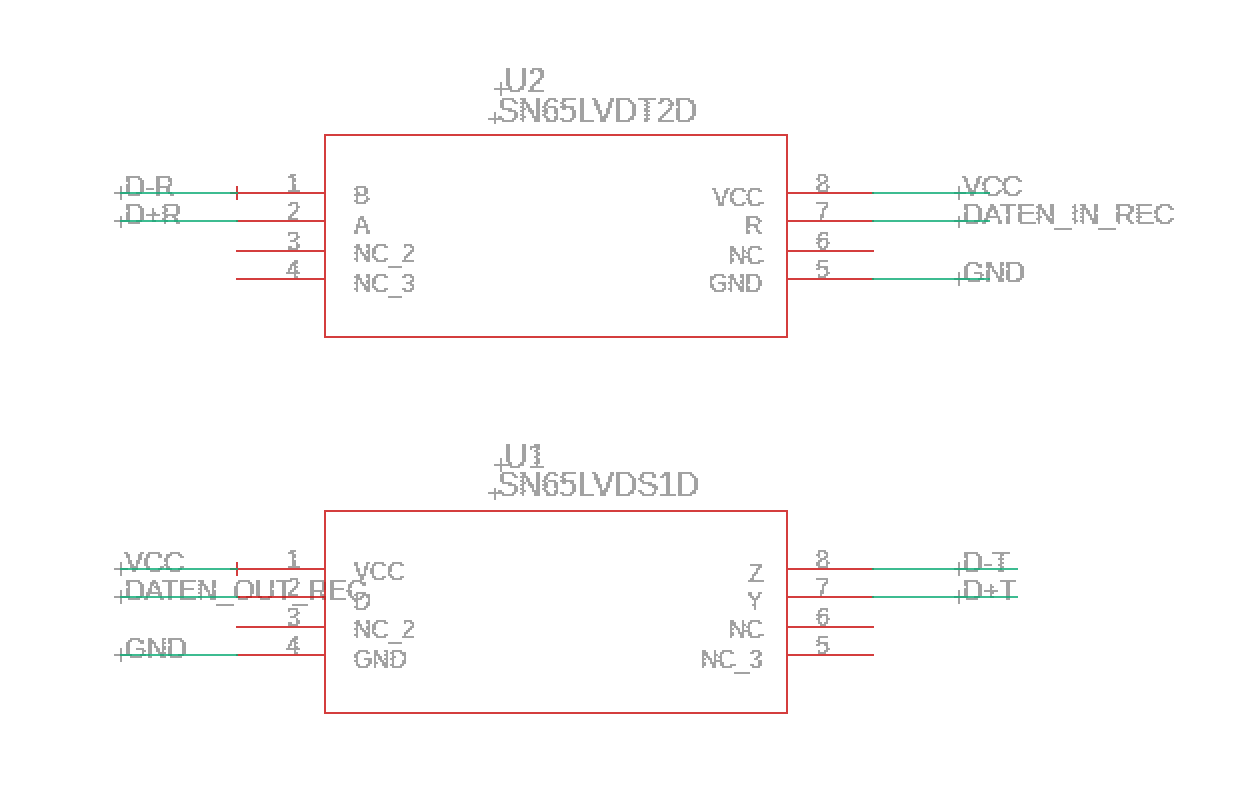
\includegraphics[width=.8\textwidth]{Bilder/BU_T_R_Bausteine.PNG}}
    \caption{Transmit-(SN65LVS1D) und Receiver(SN65LVDT2D) Bausteine }
    \label{T_R_Bausteine}
\end{figure}

\subsection{Tastatur-Modul}
Das Tastatur-Modul besteht aus 4x4 Tasten, die, wie in \ref{Tastatur} zu sehen, in einer Matrix verschaltet sind. Über die vier Ausgänge (PD2, PD3, PD4, PD5) des  ATmega werden nacheinander 
Ausgangssignale gegeben, während über die vier Eingänge (PD6, PD7, PB0, PB1) die Spalten abgefragt werden. Die Verschaltung des ATmega ist in Abb. \ref{AtMega} zu sehen. Um das korrekte Auslesen mehrerer gedrückten Tasten zu gewährleisten, werden in jedem 
Ausgangspfad Schaltdioden eingesetzt. \\
Die Datenübertragung findet über die Pins PD0 und PD1 statt.


\begin{figure}[H]
    \centering    
    \fbox{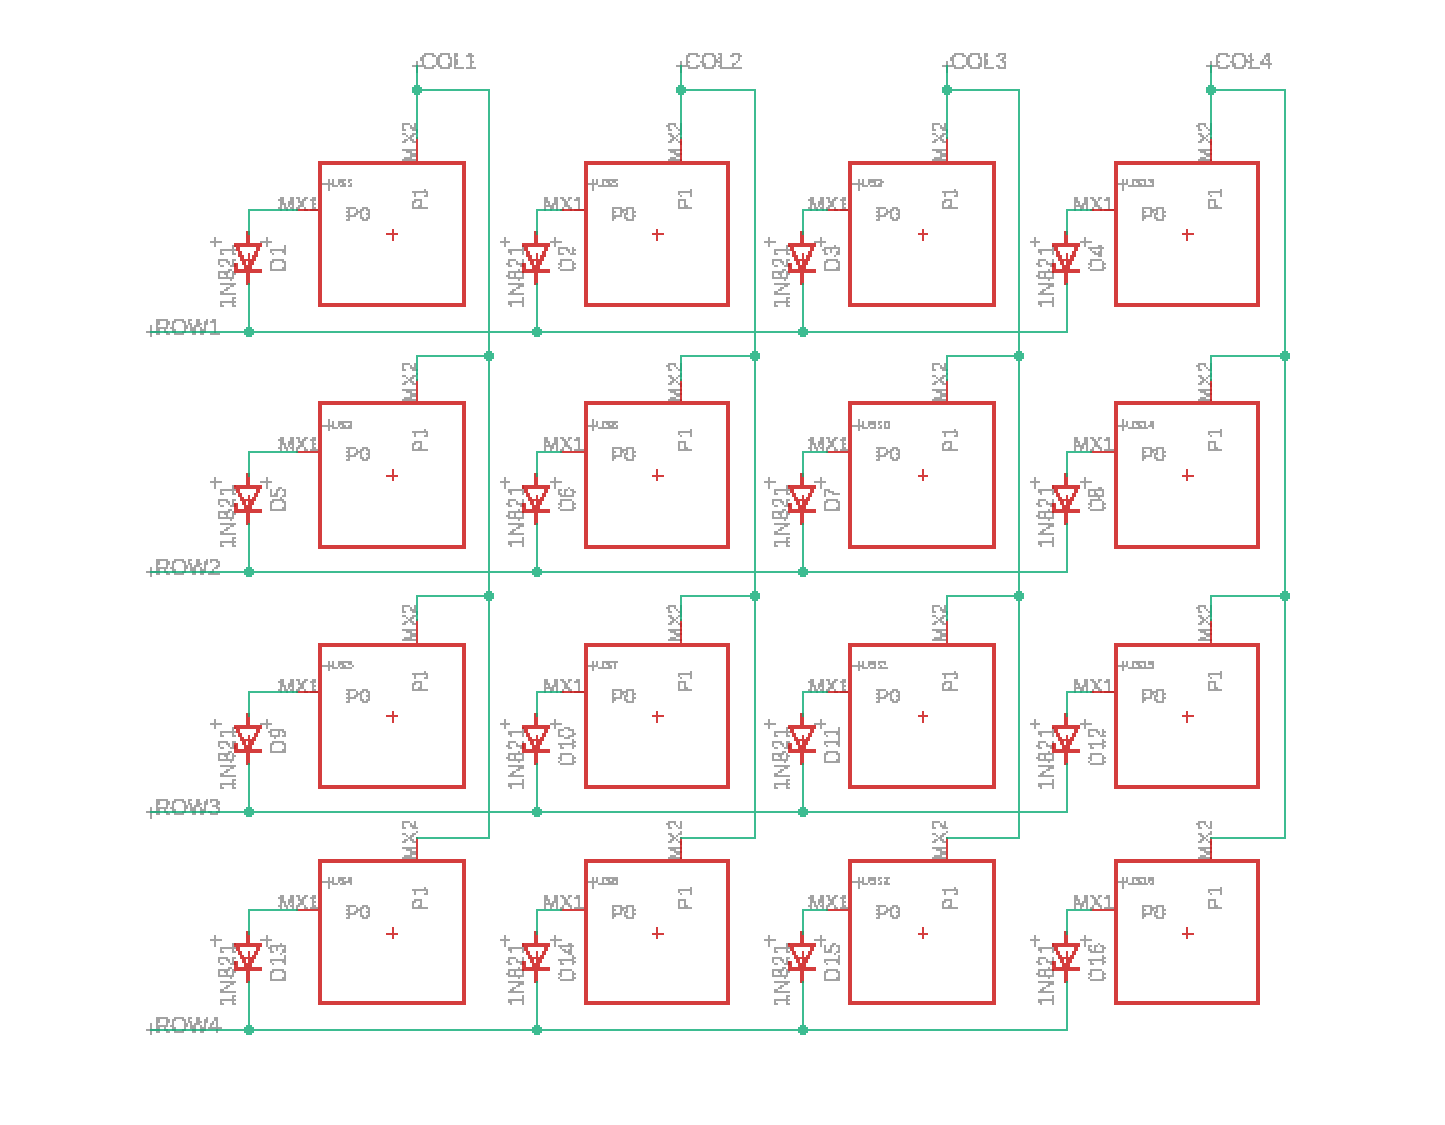
\includegraphics[width=1\textwidth]{Bilder/BU_Tastatur.PNG}}
    \caption{Tastatur Schaltung}
    \label{Tastatur}
\end{figure}


\begin{figure}[H]
    \centering    
    \fbox{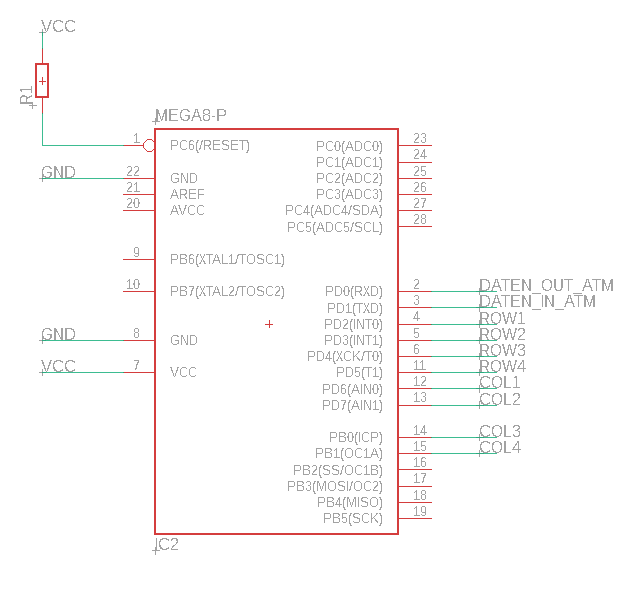
\includegraphics[width=.85\textwidth]{Bilder/AtMega.PNG}}
    \caption{ATmega Verschaltung}
    \label{AtMega}
\end{figure}


\subsection{Alternativen zum Transceiver}

Aufgrund der Probleme bei der Realisierung wurde sich dazu entschieden auf dem PCB mehrere Möglichkeiten zur differenziellen Übertragung vorzusehen 
und über Jumper schalten zu können. 
Es wird die folgenden Möglichkeiten geben:

\begin{itemize}
\item nur die Transmit/Receive ICs zu verwenden,
\item die Transmit/Receive ICs mit zusätzlichen Optokopplern zu verwenden,
\item die Optokoppler mit diskret aufgebautem Invertierern und
\item das Umschalten auf eine Lochrasterplatine, andere Testschaltungen/Testbausteine
\end{itemize}



\begin{figure}[H]
    \centering    
    \fbox{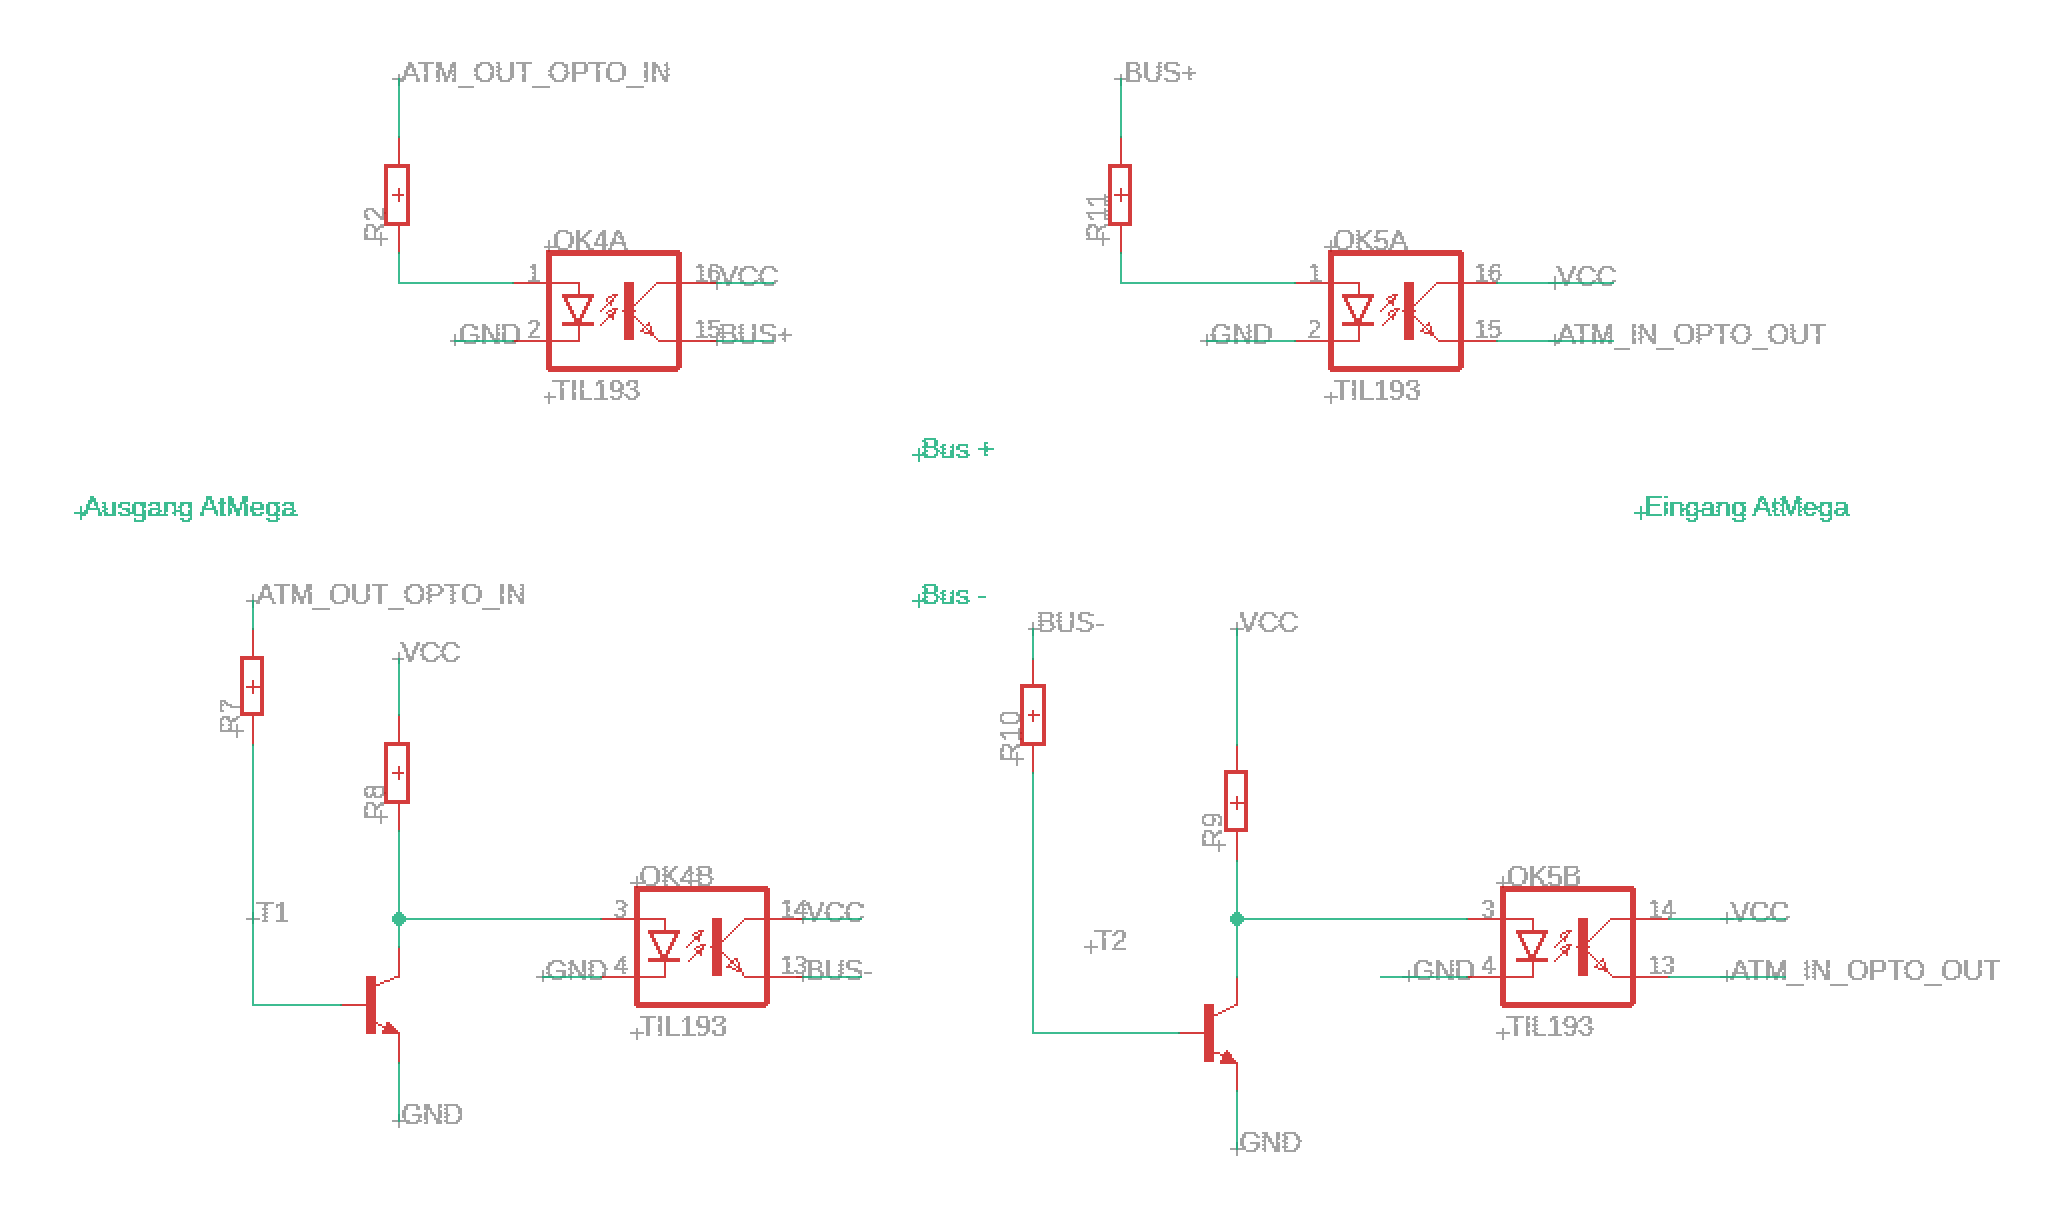
\includegraphics[width=1\textwidth]{Bilder/BU_Optokoppler.PNG}}
    \caption{Optokoppler Schaltung}
    \label{Optokoppler}
\end{figure}



\newpage
\section{PCB}
In Abb. \ref{hauptmodulPCB} ist der aktuelle Stand der PCBs für das Haupt- und in Abb. \ref{TastaturmodulPCB} der des Tastaturmodul zu sehen.

\begin{figure}[H]
    \centering    
    \fbox{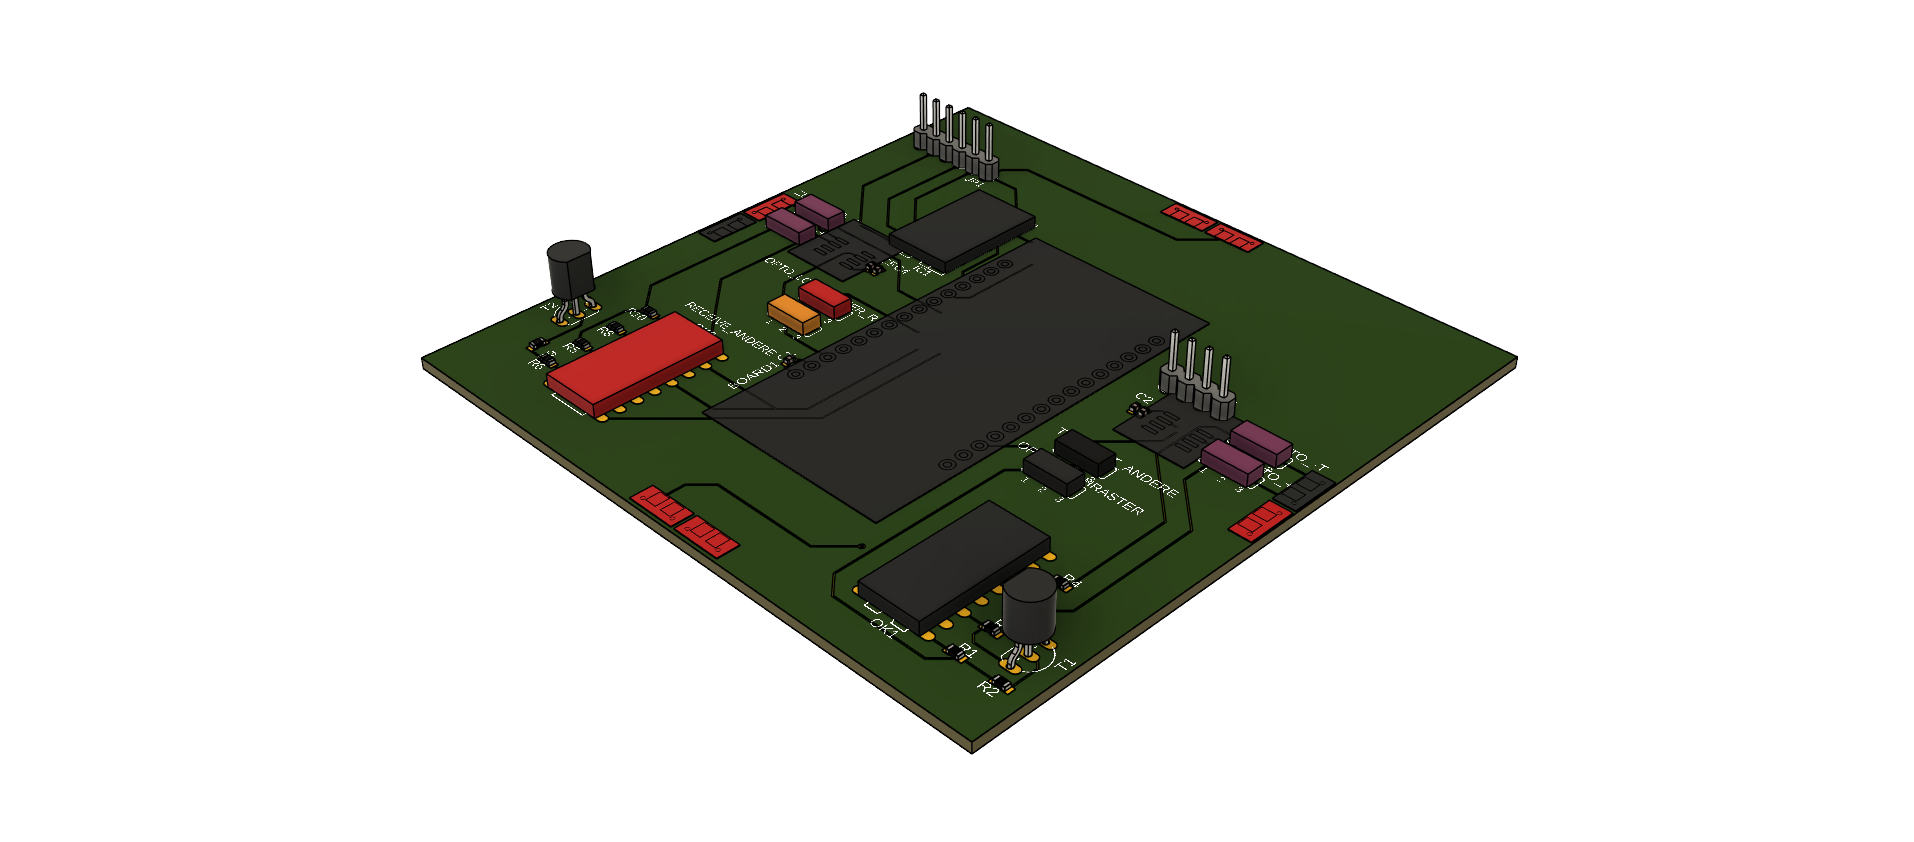
\includegraphics[width=0.85\textwidth]{Bilder/Controller.png}}
    \caption{Hauptmodul PCB}
    \label{hauptmodulPCB}
\end{figure}

\begin{figure}[H]
    \centering    
    \fbox{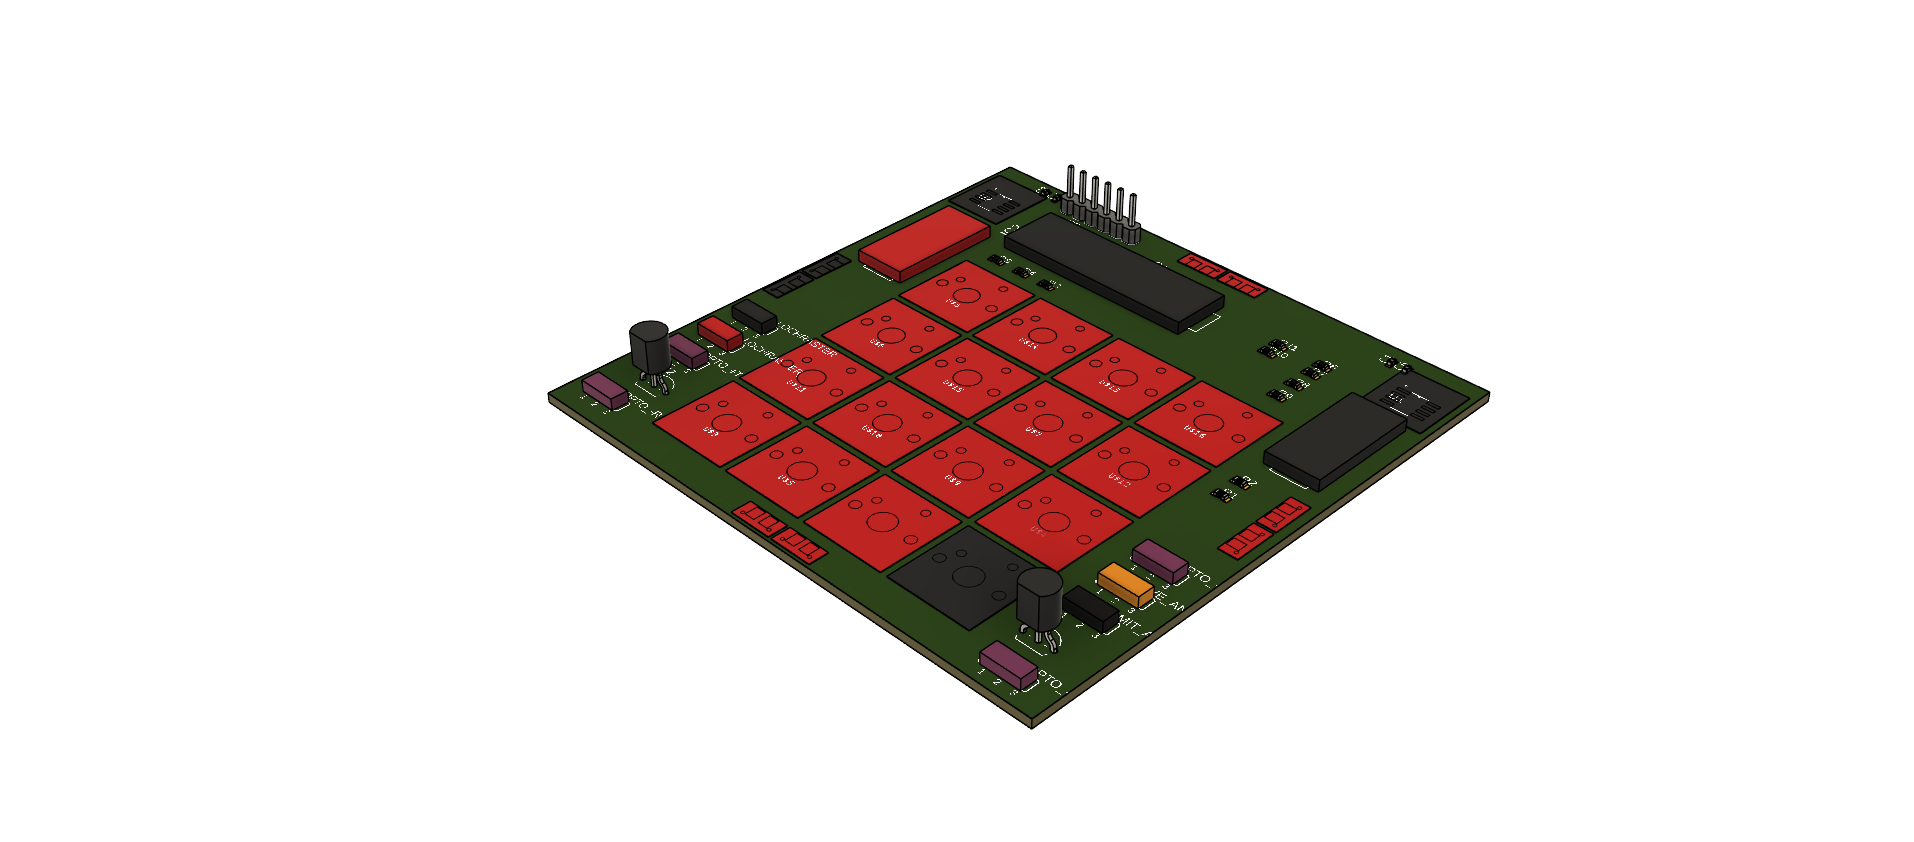
\includegraphics[width=0.85\textwidth]{Bilder/Tastatur.png}}
    \caption{Tastaturmodul PCB}
    \label{TastaturmodulPCB}
\end{figure}





